\chapter{Introduzione}

Un Lexer $\lambda $ \'e un DFA, ogni stato finale $\phi _i$ \'e associato ad una regular expression $\alpha _i$.
Una stringa $s \in L(\lambda )$, il pattern matching termina in uno stato finale $\phi _j$ ed s \'e associata ad una regular expression 
$\alpha _j$; token: ($s, \alpha _j$).

\begin{center}
	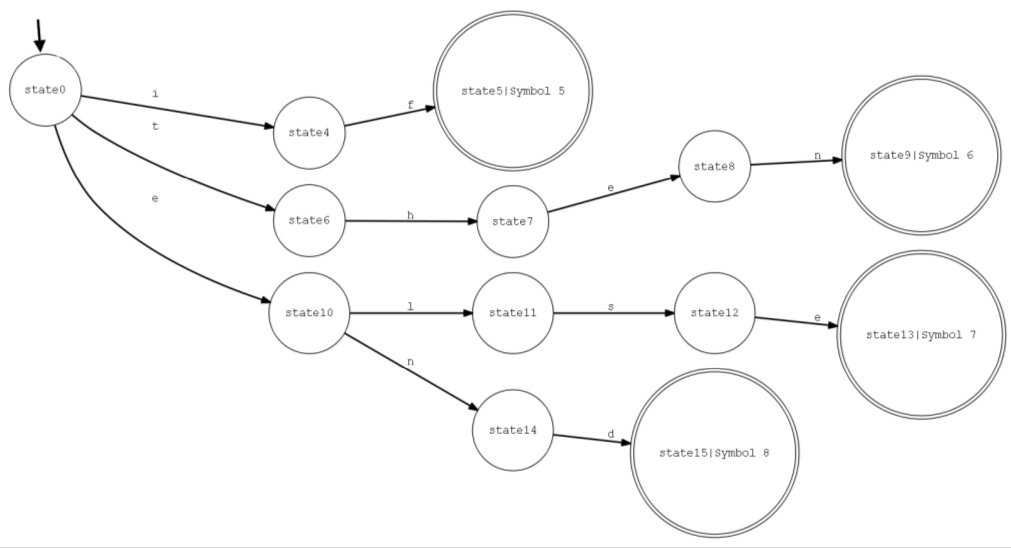
\includegraphics[scale=0.35]{Chapters/Img/c01_01.png}\\
\end{center}
	

\begin{itemize}
	\item (if, 5) \\
	\item (then, 6)\\
	\item (else, 7)\\
	\item (end, 8)\\
\end{itemize}

Data la descrizione del linguaggio che vuoi matchare lui ti genera il codice C per farlo. 

\section{Get started}
\begin{tabular}{ll}
	Windows & https://sourceforge.net/projects/winflexbison/ \\
	Linux & sudo apt-get install bison flex gcc\\
	Mac & XCode
\end{tabular}

\chapter{FLEX (Fast Lex)}
\section{Lex matching character}

\subsection{Operatori}
\begin{tabular}{ll}
	$\alpha \cdot \beta$ & concatenazione\\
	$\alpha | \beta$ & alternazione\\
	$\alpha ^+$ & una o pi\'u ripetizioni\\
	$\alpha ^*$ & zero o pi\'u ripetizioni\\
	$\alpha ?$ & 0 o 1 ripetizione\\
	$\alpha \{n,m\} | n \leq m $ & matches $\alpha$ from n to m times\\
\end{tabular}

\begin{lstlisting}
	[a-z]   	tutti i caratteri da 'a' a 'z'
	[0-9a-z_]*  tutti i caratteri n volte
	.       	ogni carattere tranne \n
	a?      	a 0 o 1 volta
	a{n,m} 		matcha a da n m volte
	a$  		a se e' alla fine di una linea
	^a  		a se e' all'inizio di una linea 
	a/b 		a iif b segue 

	[^C] 		complementare 
	[^CB]		= [^C^B] matcha bat ma non Bat o Cat 
	<<EOF>> 
	"stringa"	
	"float" | "int"
	."at" 		matches words: "cat", "rat, etc.
	[0-9a-z_] *	identificatori
\end{lstlisting}

\section{Template Lex}

\begin{lstlisting}
	%{ /* This code is copied verbatim (tale e quale) into the lexer s source code . */	%}

	/* " Named " regular expressions here . */

	%%
	/* " Anonymous " Regular expressions here . */
	%%
	
	/* This section is copied verbatim into the lexer 's source . */
\end{lstlisting}

\begin{lstlisting}
	%{ /* Copied verbatim in lexer 's source . */ %}

	Type ( " int " | " float " )
	%%
	{ Type } 	{ /* A Semantic action . */ }
	[a - z ]+ 	{ /* Another one . */ }
	%%

	int yywrap () { 
		return 1;	//if I find eof should stop lexing?
	}

	int main ( int iArgC , char ** lpszArgV ) {
		yylex (); 	// Starts lexing .
	}
\end{lstlisting}

\section{Compilare}

\begin{lstlisting}
	> flex Input.l
	> CC lex.yy.c -o Lexer.out -std=c99
	> Lexer.out < In.txt
\end{lstlisting}

\section{Variabili generate da Lex}
\begin{lstlisting}
	FILE * yyin ;		/* Default value is stdin . */
	FILE * yyout ;		/* Default value is stdout . */
	int yyleng ;		/* Number of characters read . */
	char * yytext ;		/* The buffer on which characters are copied during pattern matching*/
\end{lstlisting}

\section{Context Sensitivity (CS)}
In base al token letto devo comportarmi in modo diverso.
Ho delle \textbf{start conditions} (o start state), solo una \'e attiva. Il primo start state \'e l'\textbf{initial}.
Uno start state pu\'o essere \textbf{inclusivo} o \textbf{esclusivo}.

Da uno start state esclusivo solo re correlate ad esso sono raggiungibili.

Da uno start state inclusivo tutte le re correlate ad esso ed anche quelle non correlate agli altri start state sono raggiungibili.

\begin{lstlisting}
	%{ /* */ %}

	% x String 	// Exclusive start states
	% s Cond 	// Inclusive start states

	%%
	...
	%%
\end{lstlisting}

\section{Associare regole a stati}
Per assegnare uno start state ad una re uso \textbf{$<$NOME SS$>$}.
Per entrare in uno stato uso il comando \textbf{BEGIN}.
All inizio il lexer \'e nello stato \textbf{INITIAL}.
\begin{lstlisting}
	%{ /* */ %}

	% x Cond
	
	%%
	" \" "				{ /* Read " char . */ BEGIN Cond ;}
	< Cond >(^[ " ])+	{ /* Consume string content . */ }
	< Cond > " \" "		{ /* Read " char . */ BEGIN INITIAL ;}
	%%
\end{lstlisting}

\subsection{Stati inclusivi ed esclusivi}
\begin{lstlisting}
	%{ /* EXCLUSIVE START STATE*/ %}

	%x String Unreacheable

	%%
	" \" "					{ /* Read " char . */ BEGIN String ;}
	< String > (^[ " ])+	{ /* Consume string content . */ }
	< String > " \" "		{ /*Read " char . */ BEGIN INITIAL ;}
	< Unreacheable > "end"	{ /* Will never be matched . */ }
	%%

	%{ /* INCLUSIVE START STATE */ %}
	
	%s String
	
	%%
	" \" " 				{ /* Read " char . */ BEGIN String ;}
	< String >(^[ " ])+	{ /* Consume string content . */ }
	< String > " \" " 	{ /* Read " char . */ BEGIN INITIAL ;}
	" end "				{ /* Will be matched . */ }
	%%
\end{lstlisting}
Gli start state sono realizzati tramite uno stack, ho tre funzioni per manipolarli:
\begin{itemize}
	\item void yy push state(int NewState) //pusho in cima allo stack, equivalente a BEGIN NewState;\\
	\item void yy pop state() //fa una pop, equivalente a BEGIN;\\
	\item int yy top state() //fa la top, non esistono metacomandi per farla;\\
\end{itemize}

\section{Ambiguous Specifications}
Dati $\alpha$ e $\beta$ regular expressions talich\'e $L(\alpha ) \subset L(\beta )$, devo stare attento all'ordine in cui le scrivo, quelle pi\'u in alto hanno precedenza su quelle pi\'u in basso. 

\begin{tcolorbox}\begin{center}
	Se con molte regular expression posso arrivare in un nodo, vince quella a priorit\'a maggiore.
	Regular expressions generating constant finite languages must be placed first, or they will be obscured.
\end{center}\end{tcolorbox}

Una volta che una stringa \'e matchata viene \textbf{consumata}, le altre re non la potranno pi\'u matchare. 
Posso anche usare \textbf{REJECT} per darla in pasto alla seconda re in ordine di priorit\'a.

\begin{lstlisting}

	%{ int iCounter = 0; %}

	%%
	" abcde "	{ iCounter +=1; REJECT ;}
	" abcd "	{ iCounter +=1; REJECT ;}
	" abc "		{ iCounter +=1; REJECT ;}
	" ab "		{ iCounter +=1; REJECT ;}
	"a"			{ iCounter +=1; }
	.			{ /* Consumes the rest . */ }
	%%

	int main (){
		yylex ();
		/* iCounter = 5 when input is " abcde ". */
	}
\end{lstlisting}

\chapter{Exercises}
\section{Lex}
	Your time:
	Devise a lexer accepting a Windows file path.
	Devise a lexer accepting a Linux file path.
	Devise a lexer accepting a non regular language.